\documentclass[conference]{IEEEtran}
\usepackage{amsmath,amsfonts}
\usepackage{algorithmic}
\usepackage{algorithm}
\usepackage{array}
\usepackage[caption=false,font=normalsize,labelfont=sf,textfont=sf]{subfig}
\usepackage{textcomp}
\usepackage{stfloats}
\usepackage{url}
\usepackage{verbatim}
\usepackage{graphicx}
\usepackage{cite}
\usepackage[hypcap=false]{caption}
\usepackage{float}

% Set path for images
\graphicspath{ {./images/} }

\newenvironment{Figure}
    {\par\medskip\noindent\minipage{\linewidth}}
    {\endminipage\par\medskip}


\begin{document}

\title{Explainable Machine Learning Guided Modeling for Antennas\\
}

\author{\IEEEauthorblockN{Tyler Carr}
\IEEEauthorblockA{\textit{WiDE Laboratory} \\
\textit{Embry-Riddle Aeronautical University}\\
Daytona Beach, Florida\\
carrt12@my.erau.edu}
\and
\IEEEauthorblockN{Cameron Martinez}
\IEEEauthorblockA{\textit{WiDE Laboratory} \\
\textit{Embry-Riddle Aeronautical University}\\
Daytona Beach, Florida \\
martc114@my.erau.edu}
\and
\IEEEauthorblockN{Dr. Eduardo Rojas-Nastrucci}
\IEEEauthorblockA{\textit{WiDE Laboratory} \\
\textit{Embry-Riddle Aeronautical University}\\
Daytona Beach, Florida \\
rojase1@erau.edu}
\and
\IEEEauthorblockN{Dr. M. \.{I}lhan Akba\c{s}}
\IEEEauthorblockA{\textit{WiDE Laboratory} \\
\textit{Embry-Riddle Aeronautical University}\\
Daytona Beach, Florida \\
akbasm@erau.edu}
}

\maketitle

\begin{abstract}
    Antenna design processes require extensive electromagnetic (EM) simulation tasks that are resource-intensive, time-consuming, and prone to interruptions. Design equations are only available for predefined and limited antenna geometries. By applying a machine learning (ML) model to a limited set of data from EM simulations of a microstrip patch antenna (MPA) and leaky wave antenna (LWA), performance metrics can be predicted significantly quicker than running simulations for an extensive range of geometric variations. The model can be used for inverse design techniques, where the performance requirements are provided as input, and the model generates a geometric solution that meets those requirements. XGBRegressor was found to be the best performing model for both antenna types, with accuracies of 94.10\% and 62.71\% repsectively. Explainable ML (XAI) processes can also be applied to identify the most impactful geometric parameters, and additional simulations focusing on those parameters can be performed, creating an iterative process of intelligently generating a minimal amount of data to improve model performance This process was tested on the LWA, which saw an accuracy increase from 62.71\% to 73.43\% using XAI. 
\end{abstract}

\section{Introduction}
\subsection{Microstrip Patch Antenna}
In the realm of wireless communication, MPAs have emerged as a favored choice due to their compact size, ease of fabrication, and adaptability to various applications. Comprised of a metallic patch on a dielectric substrate, these antennas offer tunable performance characteristics such as resonant frequency, bandwidth, and radiation pattern. Despite their simplicity, predicting the behavior of MPAs involves intricate considerations of parameters like patch dimensions, substrate properties, and feeding mechanisms \cite{Patch_antennas}.

The basic design of this work is a inset-fed MPA, similar to that shown in \cite{inset_feed_pa}. It uses Rogers RT/duroid 5870, with a dielectric constant of 2.33 and dissipation factor of 0.001, for the dielectric substrate layer. There are a few crucial design parameters for the MPA, which are outlined in Figures~\ref{Planar view} and~\ref{3D view}. This design is implemented into ANSYS High-Frequency Structure Simulator (HFSS) so that it can be modeled and simulated. 

\begin{Figure}
    \centering
    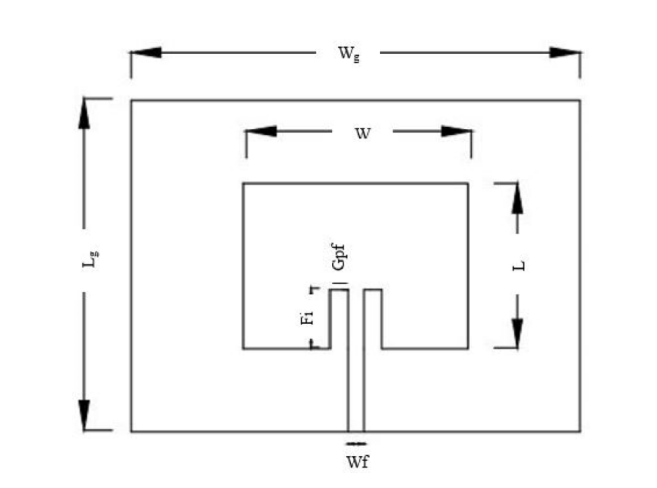
\includegraphics[width=3in]{inset_fed patch antenna.png}
    \captionof{figure}{Planar view of MPA}
    \label{Planar view}
\end{Figure}


\begin{Figure}
    \centering
    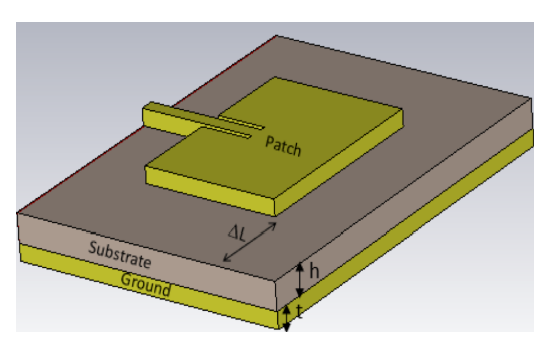
\includegraphics[width=3in]{3D patch antenna.png}
    \captionof{figure}{3-D view of MPA}
    \label{3D view}
\end{Figure}

\subsection{Leaky Wave Antenna}
The surge in wireless communication applications, spanning mobile networks, satellite communication, and Internet of Things (IoT) devices, highlights the demand for antennas adaptable to diverse operating conditions. Antenna flexibility, particularly in steering radiation patterns, has been a primary focus. While phased-array technology has shown remarkable capabilities, its complexity and size, attributed to active feeding networks, remain significant challenges. A more streamlined and cost-effective alternative is the LWA, or traveling-wave antenna. The LWA's unique wave propagation, relying on controlled electromagnetic energy leakage along its length, results in beam direction dependent on frequency. This characteristic enables beam scanning and shaping, in addition to providing high directivity and wide bandwidth \cite{LWA}. 

One common approach to achieve scanning is through a composite right/left-handed (CRLH) structure, transitioning from the backward LH region to the forward RH region with a scanning angle, \(\theta\). However, these designs typically employ substrate integrated waveguides (SIW) and metallic vias, like in \cite{crlh_siw_lwa,circular_lwa,SIW,CRLH_multivia}, which may not always be feasible, depending on size and material constraints. Alternative designs using series-fed networks of patches often have limited scanning angles, as well \cite{sfp_lwa}. 

This paper utilizes a LWA which is based upon that in \cite{CRLH_multivia}, but features a novel solution for linking the radiating patches to the bottom ground-plane, employing conductive strips positioned along the sides of the patches as illustrated in Figure~\ref{LWA}. These strips are interconnected to each unit cell via thin, conductive lines. The design also takes consideration from \cite{cpw_lwa} in its feeding mechanism, which adopts a coplanar waveguide (CPW) configuration, leveraging these side strips as a ground plane. The signal pin of the connector aligns with the central trace, which is isolated from the side ground planes by a gap and interfaces with the first radiating patch. Figure~\ref{LWA_feed} outlines the connection of these two ground planes on the feed side. This arrangement facilitates the connection of the top patches to the bottom ground plane without requiring vias, while simultaneously improving the interface between the connector and the ground plane. The design also used Rogers RO4003C, which has a dielectric constant of 3.38 and a dissipation factor of 0.0027. 

\begin{figure}[h]
\begin{center}
\noindent
    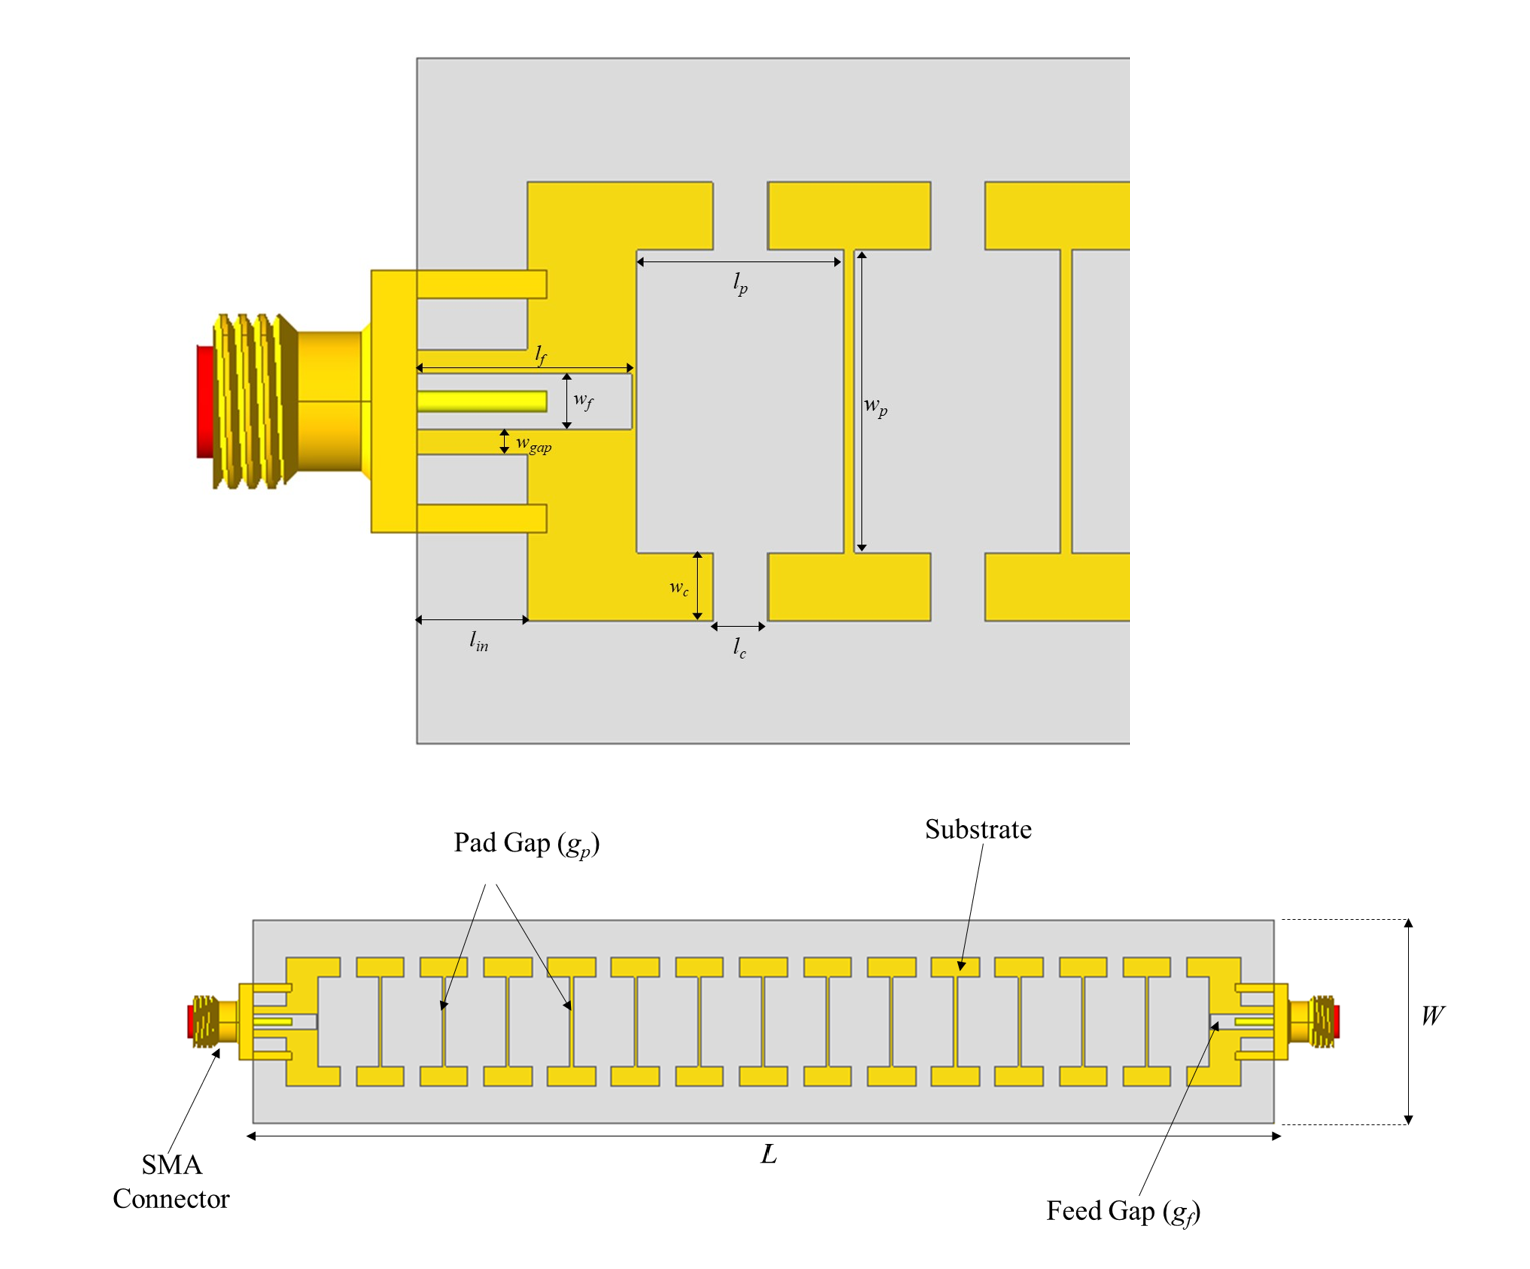
\includegraphics[width=3in]{LWA.png}
    \caption{Structure of antenna unit cell}
    \label{LWA}
\end{center}
\end{figure}

\begin{figure}[h]
\begin{center}
\noindent
    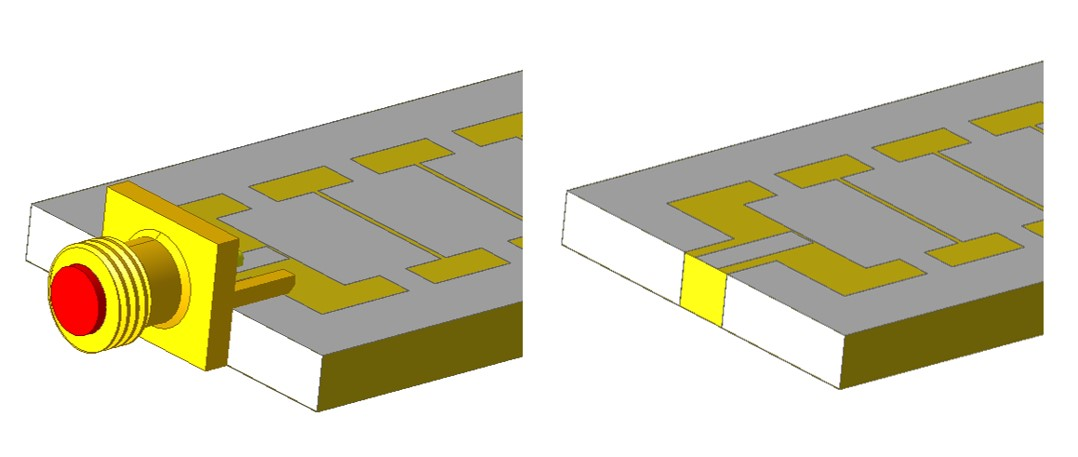
\includegraphics[width=2.5in]{Feeding Method.jpg}
    \caption{Feeding method for LWA}
    \label{LWA_feed}
\end{center}
\end{figure}

\subsection{Design and Analysis}
Traditionally, the design and analysis of antennas relied on theoretical models and electromagnetic simulation software, like HFSS, which necessitates significant computational resources and manual iterations~\cite{john_antenna_2009,ranjan_design_2023,liu_efficient_2014}. However, the integration of ML techniques has revolutionized this process by enabling rapid prediction and optimization of antenna behavior. By leveraging datasets of simulated antenna configurations, ML models can learn complex patterns and relationships, thus streamlining antenna development and enhancing performance in wireless communication systems.

One important way to evaluate antenna performance is through its scattering parameters (S-parameters), specifically its $S_{11}$. This is known as the reflection coefficient or return loss, and represents the ratio of input power to reflected power, typically expressed in decibels (dB). For passive systems, this value is always negative. A return loss of less than -10 dB demonstrates a high level of impedance matching for an antenna, and is crucial for optimizing antenna performance in terms of signal strength, bandwidth, and radiation efficiency. 

By changing the main antenna design parameters, a new geometry is created, which generates a new $S_{11}$ response. These $S_{11}$ values were specific to each geometry, and along with the parameters of that geometry, were compiled into a dataset which was then used for training and validating the ML model. Both the MPA and the LWA were put through this process. The MPA was used to prove that the process works well with a simple antenna design, and the ML model should be expected to work with very high accuracy with this antenna design. The LWA was used to test the method on a more advanced antenna design, and it is difficult to estimate what the accuracy score of the ML model will be with this antenna design. The dataset of the MPA consists of 40,905 rows, which was comprised of 405 unique geometries with $S_{11}$ values simulated across 101 frequency range values between 4GHz and 12GHz. Similarly, the dataset of the LWA consists of 23,735 rows, which was comprised of 233 unique geometries with $S_{11}$ values simulated across 101 frequency range values between 11GHz and 20GHz. Tables~\ref{antenna_dataset_p} and~\ref{antenna_design_lw} describes the relationship between the data.

\begin{table}[h]
\caption{MPA Dataset}
\begin{center}
\begin{tabular}{ |l|l|l|l| }
    \hline
    Parameter & Min & Max & Step \\ 
    \hline
    inset\_dist [mm] & 0.6 & 1.4 & 0.4 \\
    \hline
    L [mm] & 11.5 & 12.5 & 0.5 \\
    \hline
    sub\_thick [mm] & 2 & 2 & N/A \\
    \hline
    W [mm] & 14.0 & 15.6 & 0.8 \\
    \hline
    W0 [mm] & 2.5 & 3.5 & 0.5 \\
    \hline
    y0 [mm] & 3.0 & 5.0 & 0.5 \\
    \hline
    Freq [GHz] & 4.0 & 12.0 & 0.08 \\
    \hline
\end{tabular}
\end{center}
\label{antenna_dataset_p}
\end{table}


\begin{table}[h]
\caption{LWA Dataset}
\begin{center}
\begin{tabular}{ |l|l|l|l| }
    \hline
    Parameter & Min & Max & Step \\ 
    \hline
    cpw\_in [mm] & 1.5 & 2.5 & 0.25 \\
    \hline
    feed\_l [mm] & 3.25 & 4.25 & 0.25 \\
    \hline
    patch\_l [mm] & 3.25 & 4.25 & 0.25 \\
    \hline
    cpw\_g [mm] & 0.12 & 0.36 & 0.06 \\
    \hline
    Feed\_W [mm] & 0.5 & 2.0 & 0.5 \\
    \hline
    ground\_w [mm] & 0.5 & 1.5 & 0.5 \\
    \hline
    patch\_ground\_w [mm] & 0.5 & 1.5 & 0.5 \\
    \hline
    patch\_w [mm] & 4.5 & 5.0 & 0.25 \\
    \hline
    Freq [GHz] & 11.0 & 20.0 & 0.09 \\
    \hline
\end{tabular}
\end{center}
\label{antenna_design_lw}
\end{table}

There is a lot of research available on the topic of how different types of models can be useful in antenna design optimization. Liu et al.~and Li et al.~both proposed methods involving an evolutionary search mechanism~\cite{liu_efficient_2014,li_adaptive_2023}. He et al.~combined an artificial neural network (ANN) with a simulated annealing algorithm of a wideband patch antenna with four geometric parameters~\cite{10318051}. There are various other papers that compared the $R^2$ and RMSE scores of different regression models on a variety of antennas, such as an ultra-wideband, dual-port multi-in multi-out (MIMO), and THz antennas. These models include Linear, Decision Tree, Random Forest, XGBoost, K-nearest neighbors (KNN), Lasso, Ridge, Bayesian Linear, Gaussian Process, Support Vector, and ANN. The results of which model performed the best varied, and included KNN, Random Forest, and Linear~\cite{9119820,ranjan_ultra-wideband_2022,ranjan_design_2023,sharma_machine_2020,jain_estimation_2022,jain_design_2024,haque_machine_2023,m_el-kenawy_optimized_2022}. The above examples have proven that applying ML to antenna geometry optimization can decrease both the amount of time taken and the computational expensiveness when compared to typical EM simulations.

There has been less research performed on the topics of retrieving antenna geometries when given desired performance and frequency range, and applying XAI to the problem. All of the research found for the first topic appears to follow the same pattern of reversing the inputs and outputs of the respective model, using EM parameters such as gain of $S_{11}$ as inputs and using geometry parameters as outputs. Xiao et al.~applied an inverse extreme learning machine (ELM) and an ANN in an attempt to solve this problem~\cite{9063448,XiaoLi-Ye2021IANN}. Some other methods that were observed were inverse deep neural networks (DNN)~\cite{wu_ai_2024,zhang_inverse_2023}, invertable neural networks~\cite{yu_design_2020}, and more examples of ANNs~\cite{yuan_multibranch_2020}. For the XAI topic, Yeung et al.~explored applying XAI to identify important spatial regions in nanophotonic structures and photonic devices in order to optimize their design for a specific functionality~\cite{YeungChristopher2020EtBo,YeungChristopher2022EAOP}. Despite being a different problem that XAI is being applied to, this same concept is used in this approach. 

This proposed method takes a different approach to inverting the problem that allows for an additional layer of XAI. After a model was chosen, instead of achieving an inverse model by reversing the inputs and outputs of the model, predictions were made for a generated dataset that included every single possible geometry and frequency combination, which were then made to be searchable. The goal was to output optimized antenna geometries with explanations when given a $S_{11}$ and frequency range faster, while still achieving a similar result as a more complex model. The ML model accuracy was improved by applying XAI analysis on the most impactful geometric parameters. 


\section{Methodology}
Making up the generated dataset that will be searched to find the optimal antenna geometry are all possible combinations of geometric parameters and frequencies that are outlined in Tables~\ref{antenna_dataset_p} and~\ref{antenna_design_lw}. This added up to a total of 9,720 unique geometries for the MPA and 327,892 for the LWA. The simulated $S_{11}$ values for each antenna were used for the original simulated values since they were already given, and predictions were generated for the rest of the geometry and frequency combinations. This new dataset added up to a total of 981,720 and 33,117,092 rows for the MPA and LWA respectively.

In order to determine the optimal antenna geometry, a ML model was employed. This regression model was trained separately for each antenna with a supervised learning method using the dataset of simulated data. The model was then used to make predictions on all of the combinations of geometric features. The generated dataset with predictions can be searched by specifying the desired $S_{11}$ value and a frequency range that the antenna should operate within. Antenna geometries that match the search are returned, which saves significant time that would be required in a traditional antenna optimization method to set up and perform additional simulations. When seeking an optimal geometry between a certain frequency range, the geometries that result in the $S_{11}$ prediction with the lowest maximum $S_{11}$ would be chosen.


\subsection{Metrics}
In order to determine if a $S_{11}$ value was predicted accurately or not, a tolerance was utilized. The tolerance is the maximum deviation from the true value that is allowed, and the prediction is considered accurate if it is within the tolerance. This concept is used when calculating the score of a model~\eqref{eq:tolerance}, with $\epsilon$ being tolerance, $\hat{y_i}$ being the $i$th $S_{11}$ prediction, $y_i$ being the $i$th true $S_{11}$ value, and $n$ being the count of data points. The tolerance is assumed to be one when calculating all scores.

Two other common metrics to compare algorithm performance in addition to the tolerance mentioned above are the $R^2$ score~\eqref{eq:rsquared} and the Root Mean Squared Error (RMSE)~\eqref{eq:rmse}~\cite{shcherbakov_survey_2013}. The model comparisons in~\cite{haque_machine_2023,m_el-kenawy_optimized_2022,ranjan_ultra-wideband_2022,sharma_machine_2020,jain_estimation_2022,jain_design_2024} also used these same metrics to compare regression ML algorithms in their work as well. The $R^2$ score represents how well the regression line fit to the data, and the RMSE represents the difference between the predicted and true values.

\begin{figure}[h]
    \begin{equation}
        \text{Score} = \frac{1}{n} \sum_{i=1}^{n}(\left|\hat{y_i} - y_i\right| \leq \epsilon)
        \label{eq:tolerance}
    \end{equation}
    \begin{equation}
        R^2 = 1 - \frac{\sum_{i}(\hat{y_i} - \bar{y})^2}{\sum_{i}(y_i - \bar{y})^2}
        \label{eq:rsquared}
    \end{equation}
    \begin{equation}
        {RMSE} = \sqrt(\frac{1}{n} \sum_{i=1}^{n}(y_i - \hat{y}_i)^2)
        \label{eq:rmse}
    \end{equation}
    \caption{Evaluation Metrics}
\end{figure}



\subsection{Preprocessing}
Preprocessing needed to be performed on the data features before using them with any model. Firstly, the dataset was split into training and testing sets, with 20\% being reserved for testing and comparing the performance of the models, and the remaining 80\% used to train the models. A standardized scaler was then used to standardize the geometries and frequencies by removing the mean and dividing each value by the standard deviation. This is to ensure the values all have the same scale to improve model performance~\cite{9119820}. 


\subsection{Comparing Models}
Two different libraries were compared in order to determine the best model for this type of dataset. The first library that was used is TensorFlow, which was used to create a DNN~\cite{tensorflow2015-whitepaper}. The performance of the DNN was compared to many of Scikit-learn's regression models~\cite{scikit-learn}.

To keep the comparison between the algorithms fair, all preprocessing steps were performed in the same way when comparing the performance of different libraries and algorithms. When splitting the dataset into training and testing portions, the dataset was split with the same random state, meaning that every model received the same random subset of data for training. Additionally, the models were evaluated in the same way using the same performance metrics between the different libraries. All of the following were performed on the same machine to eliminate the possibility of hardware anomalies. The machine that was used contained an Intel i9-10900X 3.70 GHz CPU with 64 GB RAM and a NVIDIA GeForce RTX 3090 graphics card. 


\subsection{TensorFlow}
TensorFlow was used to create a DNN, which is useful for large datasets. The main benefit of a DNN is that it automatically figures out the most important correlations between features for you. 

The hyperparameters of the DNN were tuned in an attempt to both improve the accuracy and reduce the error rate of the model. This was done by adjusting various hyperparameters of the model, including the number of layers in the network, the rate at which the model learns, and the unit of each layer, which represents the number of neurons and outputs. This was done using a randomized searching method provided by Keras Tuner~\cite{omalley2019kerastuner}. In typical grid search hyperparameter tuning, the search space grows too large to be feasibly tested fairly quickly. With the randomized search method, a random subset of hyperparameter combinations can be tested. The most optimal results are not guaranteed, but it can get relatively close~\cite{meanti_efficient_2022}. 


\subsection{Scikit-learn}
Scikit-learn is another popular ML library where the typical use case is smaller datasets with feature extraction already having been performed. There are a multitude of regression models provided by Scikit-learn. The models that were analyzed in this test were RandomForestRegressor, GradientBoostingRegressor, AdaBoostRegressor, CatBoostRegressor, XGBRegressor, and DecisionTreeRegressor.

Similarly to with TensorFlow, a randomized search was used to determine the best hyperparameters for each model's use case. Once the optimization was performed, all of the best models had their performance compared using the same metrics. 

\subsection{Model Performance Analysis}
After the best library is determined and the best model is chosen from that library, a manual analysis was performed using a number of random unique antenna geometry configurations for both antenna designs. The geometries selected have never been seen by the simulation, training set, or testing set. They then have both their simulated and predicted $S_{11}$ values for the entire frequency range from the HFSS and best chosen model compared. This process is done in order to narrow in on random samples of actual data to check that the model is performing comparably to the simulation software. The geometric parameters of the chosen unseen geometries are recorded in Table~\ref{unseen_geometries_p} and Table~\ref{unseen_geometries_lw}.

\begin{table}[h]
\caption{Unseen Geometry Parameters}
\begin{center}
\begin{tabular}{ |l|l|l|l|l|l|l| }
    \hline
    ID & 1 & 2 & 3 & 4 & 5 & 6 \\ 
    \hline
    inset\_dist [mm] & 0.6 & 0.6 & 1.0 & 1.4 & 1.4 & 1.4 \\
    \hline
    L [mm] & 11.5 & 12.0 & 12.0 & 11.5 & 11.5 & 11.75 \\
    \hline
    sub\_thick [mm]  & 2.0 & 2.0 & 2.0 & 2.0 & 2.0 & 2.0 \\
    \hline
    W [mm]  & 14.8 & 14.8 & 15.6 & 15.6 & 15.4 & 15.4 \\
    \hline
    W0 [mm] & 2.5 & 2.75 & 3.5 & 3.5 & 3.5 & 3.5 \\
    \hline
    y0 [mm] & 4.25 & 4.5 & 4.25 & 4.25 & 4.5 & 4.75 \\
    \hline
\end{tabular}
\end{center}
\label{unseen_geometries_p}
\end{table}    

\begin{table}[h]
\caption{Unseen Geometry Parameters}
\begin{center}
\begin{tabular}{ |l|l|l|l|l|l|l| }
    \hline
    ID & 1 & 2 & 3 & 4 & 5 & 6 \\
    \hline
    cpw\_in [mm] & 2.5 & 1.75 & 1.75 & 1.75 & 2.5 & 2.5 \\
    \hline
    feed\_l [mm] & 3.25 & 3.25 & 3.5 & 4 & 3.75 & 4 \\
    \hline
    patch\_l [mm] & 3.5 & 3.25 & 3.5 & 4 & 3.75 & 4.25 \\
    \hline
    cpw\_g [mm] & 0.18 & 0.3 & 0.3 & 0.12 & 0.36 & 0.24 \\
    \hline
    Feed\_W [mm] & 1.25 & 0.5 & 1.25 & 1.25 & 0.5 & 1.75 \\
    \hline
    ground\_w [mm] & 0.5 & 0.75 & 1 & 1.25 & 1.5 & 1 \\
    \hline
    patch\_ground\_w [mm] & 0.5 & 1 & 0.5 & 1.5 & 1 & 1.25 \\
    \hline
    patch\_w [mm] & 5 & 5 & 5 & 4.75 & 5 & 4.5 \\
    \hline
\end{tabular}
\end{center}
\label{unseen_geometries_lw}
\end{table}    
    



\subsection{Explainability}
SHAP, an open-source game theoretic approach to XAI, is used to demonstrate how much each geometric parameter swayed the predicted $S_{11}$ value~\cite{NIPS2017_7062}. Beeswarm plots are used to enhance understanding of the relationship between the geometric parameters and the $S_{11}$ values by showing which parameters have the highest impact on the prediction being made for the model as a whole, and in which way they are swaying the prediction. By determining which geometric features have the highest impact on the predictions, additional simulations can be simulated by focusing on these features to minimize the amount of data that needs to be simulated. Waterfall plots can also be created for individual predictions to analyze the highest contributing features to that particular prediction.

\subsection{Manufacturing Antenna}
After performing all of the above steps, a graphical user interface (GUI) was created to allow a user to pick a potential antenna geometry for a desired $S_{11}$ and operational frequency range using the predictions that were generated. The geometry was chosen before the additional training was performed using the knowledge of the best parameters from XAI. The geometry was then run through HFSS, and the performance across the frequency range was compared between the simulated, values, the predicted values, and the actual measured values. 


\section{Results}
\subsection{Library and Model Comparison with the MPA}
Both antennas were used to test and compare the performance of models from the two different libraries: TensorFlow and Scikit-learn. The best performing model was chosen from each library, and their training time, predicting time, accuracy, and RMSE were compared in order to select the best model.

The Keras Tuner search for optimal hyperparameters of the DNN provided the results in Table~\ref{keras_best_params}. This was tested for both the MPA and the LWA. The MPA was found to work best with a smaller DNN consisting of two layers, where the LWA performed best with only one. The optimal learning rate was similar for both antennas, with the MPA having the higher learning rate. The DNNs were able to predict $S_{11}$ values with an error tolerance of~$\pm$1dB for the MPA and LWA with a 84.17\% and 27.26\% accuracy respectively. These accuracies are not desirable, and might be an indicator that a DNN is too complex for this job.

\begin{table}[h]
\caption{Keras Tuner Best Hyperparameters}
\begin{center}
\begin{tabular}{ |l|l|l|l| }
    \hline
    Name & Patch Value & Leaky Wave Value \\ 
    \hline
    num\_layers & 2 & 1 \\  
    \hline
    units\_0 & 256 & 224 \\
    \hline
    units\_1 & 32 & N/A \\
    \hline
    learning\_rate & 0.0841 & 0.0522 \\
    \hline
\end{tabular}
\end{center}
\label{keras_best_params}
\end{table}

Figure~\ref{dnn_loss_graph} shows how the DNN's loss decreased as the number of epochs increased for both the MPA and the LWA. The loss was significantly less for the MPA, which is to be expected as the model is having an easier time fitting to the simpler antenna design. The fact that this graph shows both the training and testing decreasing shows that the model is converging. Additionally, the model is not overfitting. 

\begin{Figure}
    \centering
    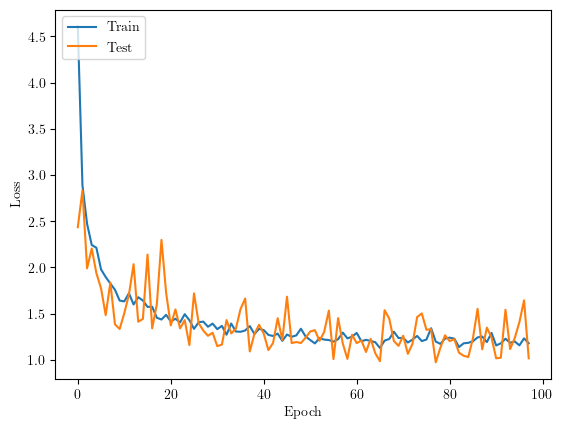
\includegraphics[width=3in]{loss}
    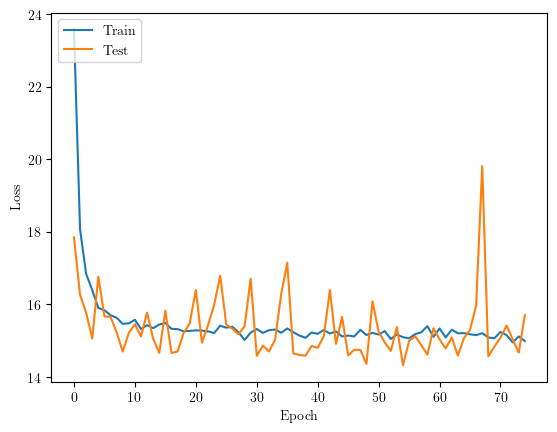
\includegraphics[width=3in]{loss_lw}
    \captionof{figure}{DNN Loss Graph for MPA and LWA}
    \label{dnn_loss_graph}
\end{Figure}

Each of the Scikit-learn regression models performed differently than one another. After performing a randomized search for the best hyperparameters for each type of model, the score of the best configuration of each model was reported alongside the $R^2$ and RMSE scores in Tables~\ref{comparing_sklearn_p} and~\ref{comparing_sklearn_lw}. The tables are sorted by best to worst performance by score, RMSE, and $R^2$. The goal is to have the accuracy and $R^2$ closest to one, and the RMSE closest to zero. It's clear by looking at the tables that XGBRegressor is the best performing model for both antennas. It has the highest accuracy and the lowest RMSE, which proves that its predictions had the least distance from the actual $S_{11}$ values. 


\begin{table}[h]
    \caption{Scikit-learn Results for MPA}
    \begin{center}
    \begin{tabular}{ |l|l|l|l| }
        \hline
        Model Type & Accuracy within~$\pm$1dB & RMSE & $R^2$ \\ 
        \hline
        XGBRegressor & 0.9410 & 0.7330 & 0.9651 \\  
        \hline
        RandomForestRegressor & 0.9286 & 0.7717 & 0.9614 \\
        \hline  
        GradientBoostingRegressor & 0.9012 & 0.9950 & 0.9357 \\
        \hline
        CatBoostRegressor & 0.8969 & 0.9949 & 0.9358 \\    
        \hline
        DecisionTreeRegressor & 0.8808 & 1.1082 & 0.9202 \\  
        \hline
        AdaBoostRegressor & 0.8523 & 1.1956 & 0.9072 \\  
        \hline
    \end{tabular}
    \end{center}
    \label{comparing_sklearn_p}
    \end{table}
    
    \begin{table}[h]
    \caption{Scikit-learn Results for LWA}
    \begin{center}
    \begin{tabular}{ |l|l|l|l| }
        \hline
        Model Type & Accuracy within~$\pm$1dB & RMSE & $R^2$ \\ 
        \hline
        XGBRegressor & 0.6271 & 2.686 & 0.7819 \\  
        \hline
        RandomForestRegressor & 0.6164 & 2.613 & 0.7934 \\
        \hline  
        GradientBoostingRegressor & 0.5805 & 2.760 & 0.7697 \\
        \hline
        DecisionTreeRegressor & 0.5123 & 3.276 & 0.6754 \\  
        \hline
        CatBoostRegressor & 0.3691 & 3.369 & 0.6567 \\    
        \hline
        AdaBoostRegressor & 0.3461 & 3.665 & 0.5938 \\  
        \hline
    \end{tabular}
    \end{center}
    \label{comparing_sklearn_lw}
    \end{table}

The learning curve in Figure~\ref{learning_curve} demonstrates the tradeoff between variance and bias when training the ML model. The learning curve shows that the RMSE decreases significantly as more training data is added to the model, which means that the model is fitting to the data. However, because the validation and the training sets never converge and have a large distance between them, our model has high variance. This means that the model is being given too many features when compared to the amount of rows of training data available. This can be fixed by adding more training data, an idea which will be revisited in Section~\ref{sec:xai}.

\begin{Figure}
    \centering
    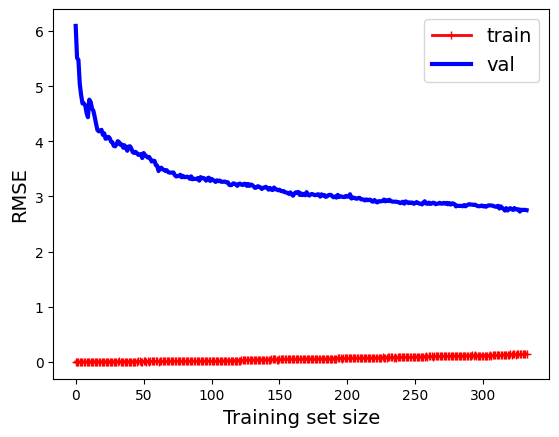
\includegraphics[width=2.5in]{images/learningcurve1.png}
    \captionof{figure}{XGBRegressor Learning Curve for LWA}
    \label{learning_curve}
\end{Figure}


When comparing the TensorFlow and Scikit-learn libraries, the same random state was used when splitting the data into training and testing portions. This ensures that each library is given a fair chance with the same set of data and the data isn't being swayed unintentionally. The TensorFlow model had 500 epochs, but only used 35 of them for the MPA and 75 for the LWA due to the early stopping criteria that was set. 

It's clear from Tables~\ref{comparing_libraries_p} and~\ref{comparing_libraries_lw} that Scikit-learn is the best choice of library for both of the antenna designs. The Scikit-learn model performed with better accuracy when predicting values with a tolerance of~$\pm$1dB, and it has a lower RMSE.

\begin{table}[h]
\caption{Comparing Libraries for MPA}
\begin{center}
\begin{tabular}{ |l|l|l| }
    \hline
    Model Type & TensorFlow & Scikit-learn \\ 
    \hline
    Training Time (s) & 273.0s & 88.0 \\  
    \hline
    Predicting Time (s) & 2.91 & 3.69 \\
    \hline
    $S_{11}$ Accuracy within~$\pm$1dB & 0.8417 & 0.9314 \\
    \hline
    RMSE & 1.5050 & 0.7851 \\
    \hline
\end{tabular}
\end{center}
\label{comparing_libraries_p}
\end{table}

\begin{table}[h]
\caption{Comparing Libraries for LWA}
\begin{center}
\begin{tabular}{ |l|l|l| }
    \hline
    Model Type & TensorFlow & Scikit-learn \\ 
    \hline
    Training Time (s) & 65.0 & 86.0 \\  
    \hline
    Predicting Time (ms) & 210.0 & 17.6 \\
    \hline
    $S_{11}$ Accuracy within~$\pm$1dB & 0.2726 & 0.6731 \\
    \hline
    RMSE & 14.237 & 2.686 \\
    \hline
\end{tabular}
\end{center}
\label{comparing_libraries_lw}
\end{table}

Figure~\ref{histogram_of_error_patch} shows how the Scikit-learn model had lower error between the predicted $S_{11}$ values and the actual $S_{11}$ values than the DNN model for the MPA. The DNN model tended to make predictions that were lower than the actual values. Additionally, Figure~\ref{actual_vs_predicted_s11_patch} demonstrates how the $S_{11}$ predictions were closer to the actual values, which is depicted by the diagonal line, for the Scikit-learn model. The DNN model had trouble predicting thet outliers. 

\begin{Figure}
    \centering
    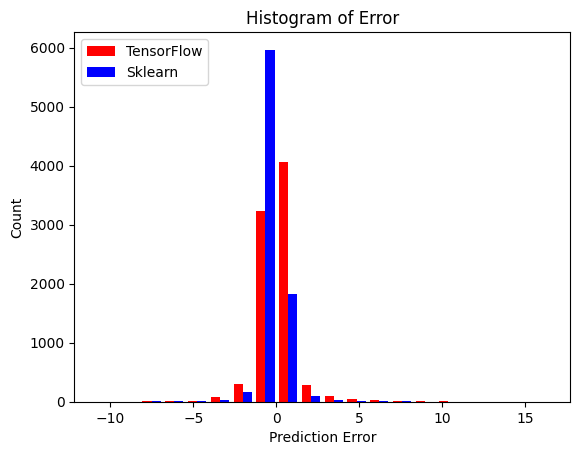
\includegraphics[width=3in]{histogram_patch}
    \captionof{figure}{Histogram of Error for MPA}
    \label{histogram_of_error_patch}
\end{Figure}

\begin{Figure}
    \centering
    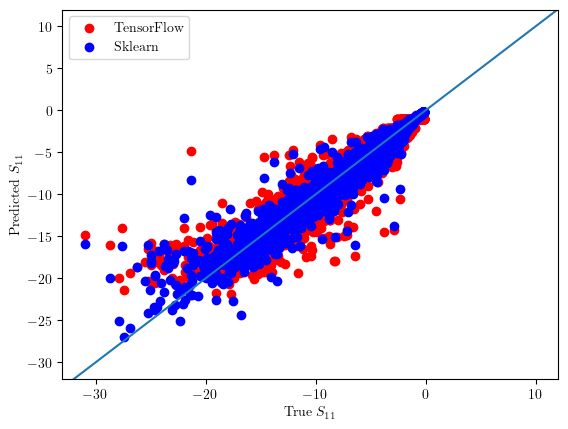
\includegraphics[width=3in]{actual_vs_predicted_s11_patch}
    \captionof{figure}{Actual vs Predicted $S_{11}$ for MPA}
    \label{actual_vs_predicted_s11_patch}
\end{Figure}

Figures~\ref{histogram_of_error_leaky_wave} and~\ref{actual_vs_predicted_s11_leaky_wave} show how the results for the LWA are similar to those of the MPA. The LWA was trained on fewer geometries and the antenna has two additional parameters, making it more complex. These facts are reflected by the poorer overall performance of both the DNN model and the Scikit-learn model. However, similarly to with the MPA, both figures prove that the Scikit-learn model makes $S_{11}$ predictions with higher accuracy than the DNN model.

\begin{Figure}
    \centering
    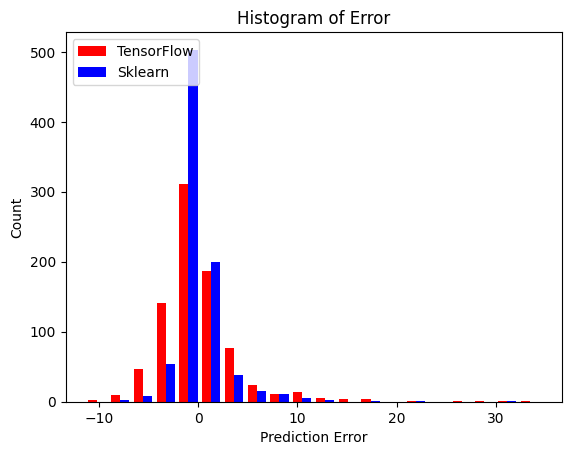
\includegraphics[width=3in]{histogram_leaky_wave}
    \captionof{figure}{Histogram of Error for LWA}
    \label{histogram_of_error_leaky_wave}
\end{Figure}

\begin{Figure}
    \centering
    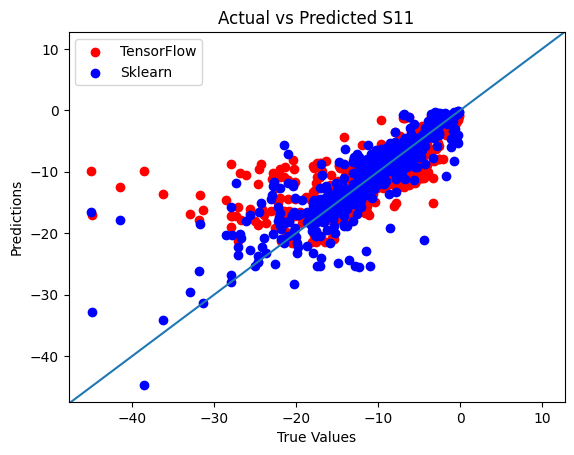
\includegraphics[width=3in]{actual_vs_predicted_s11_leaky_wave}
    \captionof{figure}{Actual vs Predicted $S_{11}$ for LWA}
    \label{actual_vs_predicted_s11_leaky_wave}
\end{Figure}

\subsection{Testing with Unseen Geometries}
For each antenna, the chosen model was given a set of six randomly selected geometries that had never been seen before by either the training set or testing set. These geometries were part of the combinations that were generated to create the dataset for optimal geometry searching, so they have also never been seen by the simulator. They were run through both the HFSS and the chosen ML model in order to obtain simulated and predicted $S_{11}$ values for the entire frequency range of the antenna. The results are shown in Figures~\ref{unseen_geometries_graph_p} and~\ref{unseen_geometries_graph_lw}, for the MPA and the LWA respecitvely. In these figures, each unseen geometry has its simulated $S_{11}$ values plotted alongside the predicted values for each frequency in the frequency range.


\begin{Figure}
    \centering
    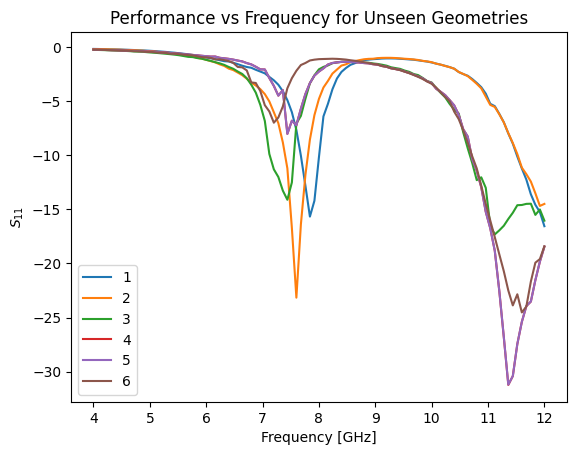
\includegraphics[width=3.25in]{unseen_geometries_freq_vs_seq}
    \captionof{figure}{Unseen Geometries for MPA}
    \label{unseen_geometries_graph_p}
\end{Figure}

\begin{Figure}
    \centering
    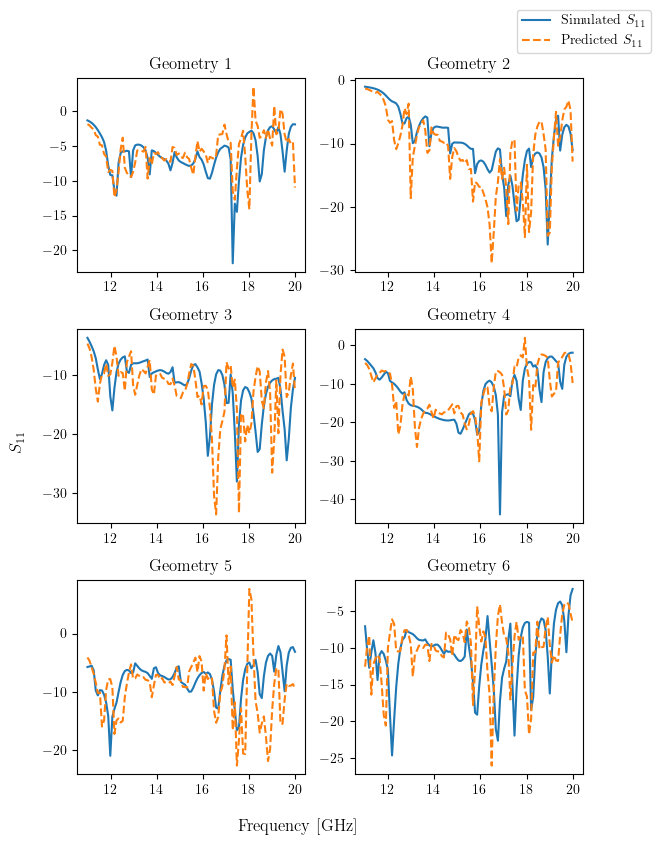
\includegraphics[width=3.25in]{unseen_geometries_freq_vs_seq_lw}
    \captionof{figure}{Unseen Geometries for LWA}
    \label{unseen_geometries_graph_lw}
\end{Figure}

For the MPA, it's interesting to note how the prediction of the $S_{11}$ values of Geometry 2 was nearly identical to the simulated values. For Geometries 3, 4, and 6, both the predicted values and the simulated values had similar dips in the curves around 7GHz and 11GHz. However, the dips were shifted to slightly lower frequency ranges for the predicted values. Additionally, for all geometries tested, the predicted $S_{11}$ values appear to follow the same trend as the simulated values, but they never reach as far low as the simulated values reach. 

While the predicted $S_{11}$ values for the LWA are obviously not nearly as accurate when compared to the simulated values, it can be observed that they follow the same general trend. There are certain areas where the predictions perform very well, particularly in Geometry 1 between 10 and 15 GHz, Geometry 2 between 18.5 and 19.5 GHz, and Geometry 5 between 13 and 17 GHz. For Geometries 1, 4, and 5, the predicted value appears to rise above zero, which should theoretically never happen. With more training data included from more simulations, the predictions will slowly become more fit to the simulated values. 


\subsection{SHAP}
\label{sec:xai}
SHAP was applied to the model as an XAI analysis tool. In order to feasibly use SHAP with the LWA dataset, a random sample of 5,000 points was used. This sample consisted of all of the geometric parameters and the frequency, and accurately captures characteristics and trends present of the entire dataset. The best performing model, which was XGBRegressor, was used with scaled data in order to interface with the SHAP primary explainer. 

    
\begin{Figure}
\centering
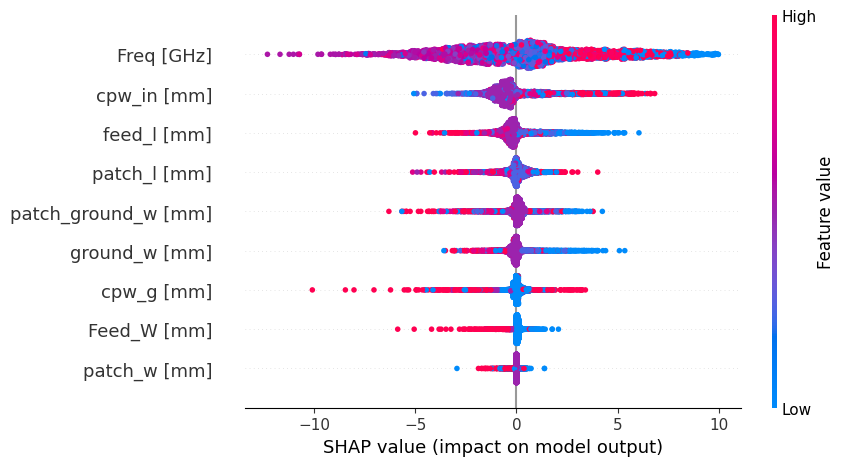
\includegraphics[width=3in]{shap_beeswarm}
\captionof{figure}{Beeswarm Plot of Features Impacting Predictions}
\label{shap_beeswarm}
\end{Figure}

Figure~\ref{shap_beeswarm} is a SHAP beeswarm plot, which demonstrates the impact that each feature had on the predictions made by the model overall for the LWA. The figure shows how frequency had a significantly higher impact on $S_{11}$ predictions than any geometric feature, which makes sense because antennas have an entirely different performance depending on what frequency is used. The other geometric parameters appear to have similar impacts on the predictions being made. $feed\_l$, $ground\_l$, and $Feed\_W$ all consistently had higher values of these features causing lower predictions to be made, and lower values causing higher predictions. The opposite was true for $cpw\_in$. For $cpw\_g$, high feature values caused both high and low predictions, but lower feature values caused the prediction to stay relatively the same. All of the other features seemed to be random and didn't have any correlation. 

From these observations, two geometric parameters were chosen as the most impactful parameters. $cpw\_g$ has a wide spread with some SHAP values reaching as far as -10, and $cpw\_in$ has a cluster that occurs the furthest away from zero. 77 more unique geometries were simulated across the frequency range, and when combined with the original 233, the accuracy increased from 0.6271 to a significantly better 0.7343. That's an accuracy increase of over 10\% that was attributed to only 77 additional geometry simulations. In addition, the RMSE and $R^2$ scores improved, with the new scores being 2.319 and 0.8336. If this process were to be repeated one or two more times, an improvement across all of the metrics is likely to be seen. 


\subsection{Finding Optimal Geometry}
A GUI was implemented using Jupyter Widgets to allow for ease of exploring different types of geometries~\cite{interactive_Jupyter_widgets}. This was implemented specifically for exploring the geometries of the LWA, but could be adapted to use with other antenna designs, such as the MPA. A user inputs a desired $S_{11}$ value and frequency range, and a graph showing predicted $S_{11}$ values for the frequency range will be plotted for the best performing geometries. This graph includes marker lines as a visual aid to show what value the $S_{11}$ predictions should be below and what frequency values the predictions should be between. The GUI allows the user to interactively explore which geometric parameters lead to a specified performance, where before this was a manual and timely process.  

\begin{Figure}
    \centering
    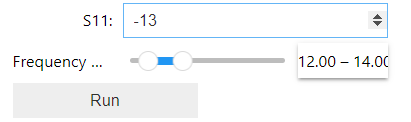
\includegraphics[width=2in]{gui_input}
    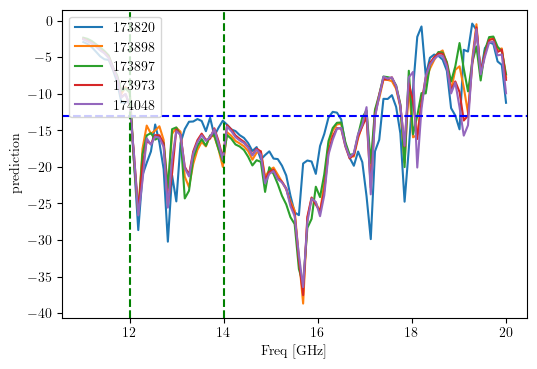
\includegraphics[width=3in]{gui_graph}
    \captionof{figure}{GUI Input and Predicted $S_{11}$ vs Frequency for Optimal Geometries}
    \label{gui}
\end{Figure}

An example of an input and the corresponding graph that is generated is shown in Figure~\ref{gui}. The specified $S_{11}$ value of -25 dB is represented by the dotted horizontal blue line, and the selected frequency range between 12.81 GHz and 13.03 GHz is represented by the two dotted vertical green lines. All of the 4 geometries that are found have predicted $S_{11}$ values within these constraints. 

\begin{table}[h]
\caption{Manufactured LWA Geometries}
\begin{center}
\begin{tabular}{ 
|l|l|l|}
    \hline
    Geometry Name & 1 & 2 \\
    \hline
    cpw\_in [mm] & 2.0 & 1.8 \\
    \hline
    feed\_l [mm] & 4.0 & 3.75 \\
    \hline
    patch\_l [mm] & 3.5 & 3.75 \\
    \hline
    cpw\_g [mm] & 0.18 & 0.24 \\
    \hline
    Feed\_W [mm] & 2.0 & 2.0 \\
    \hline
    ground\_w [mm] & 1.5 & 0.75 \\
    \hline
    patch\_ground\_w [mm] & 1.25 & 1.25 \\
    \hline
    patch\_w [mm] & 4.5 & 5.0 \\
    \hline
\end{tabular}
\end{center}
\label{manufactured_geometries_list}
\end{table}

\begin{Figure}
    \centering
    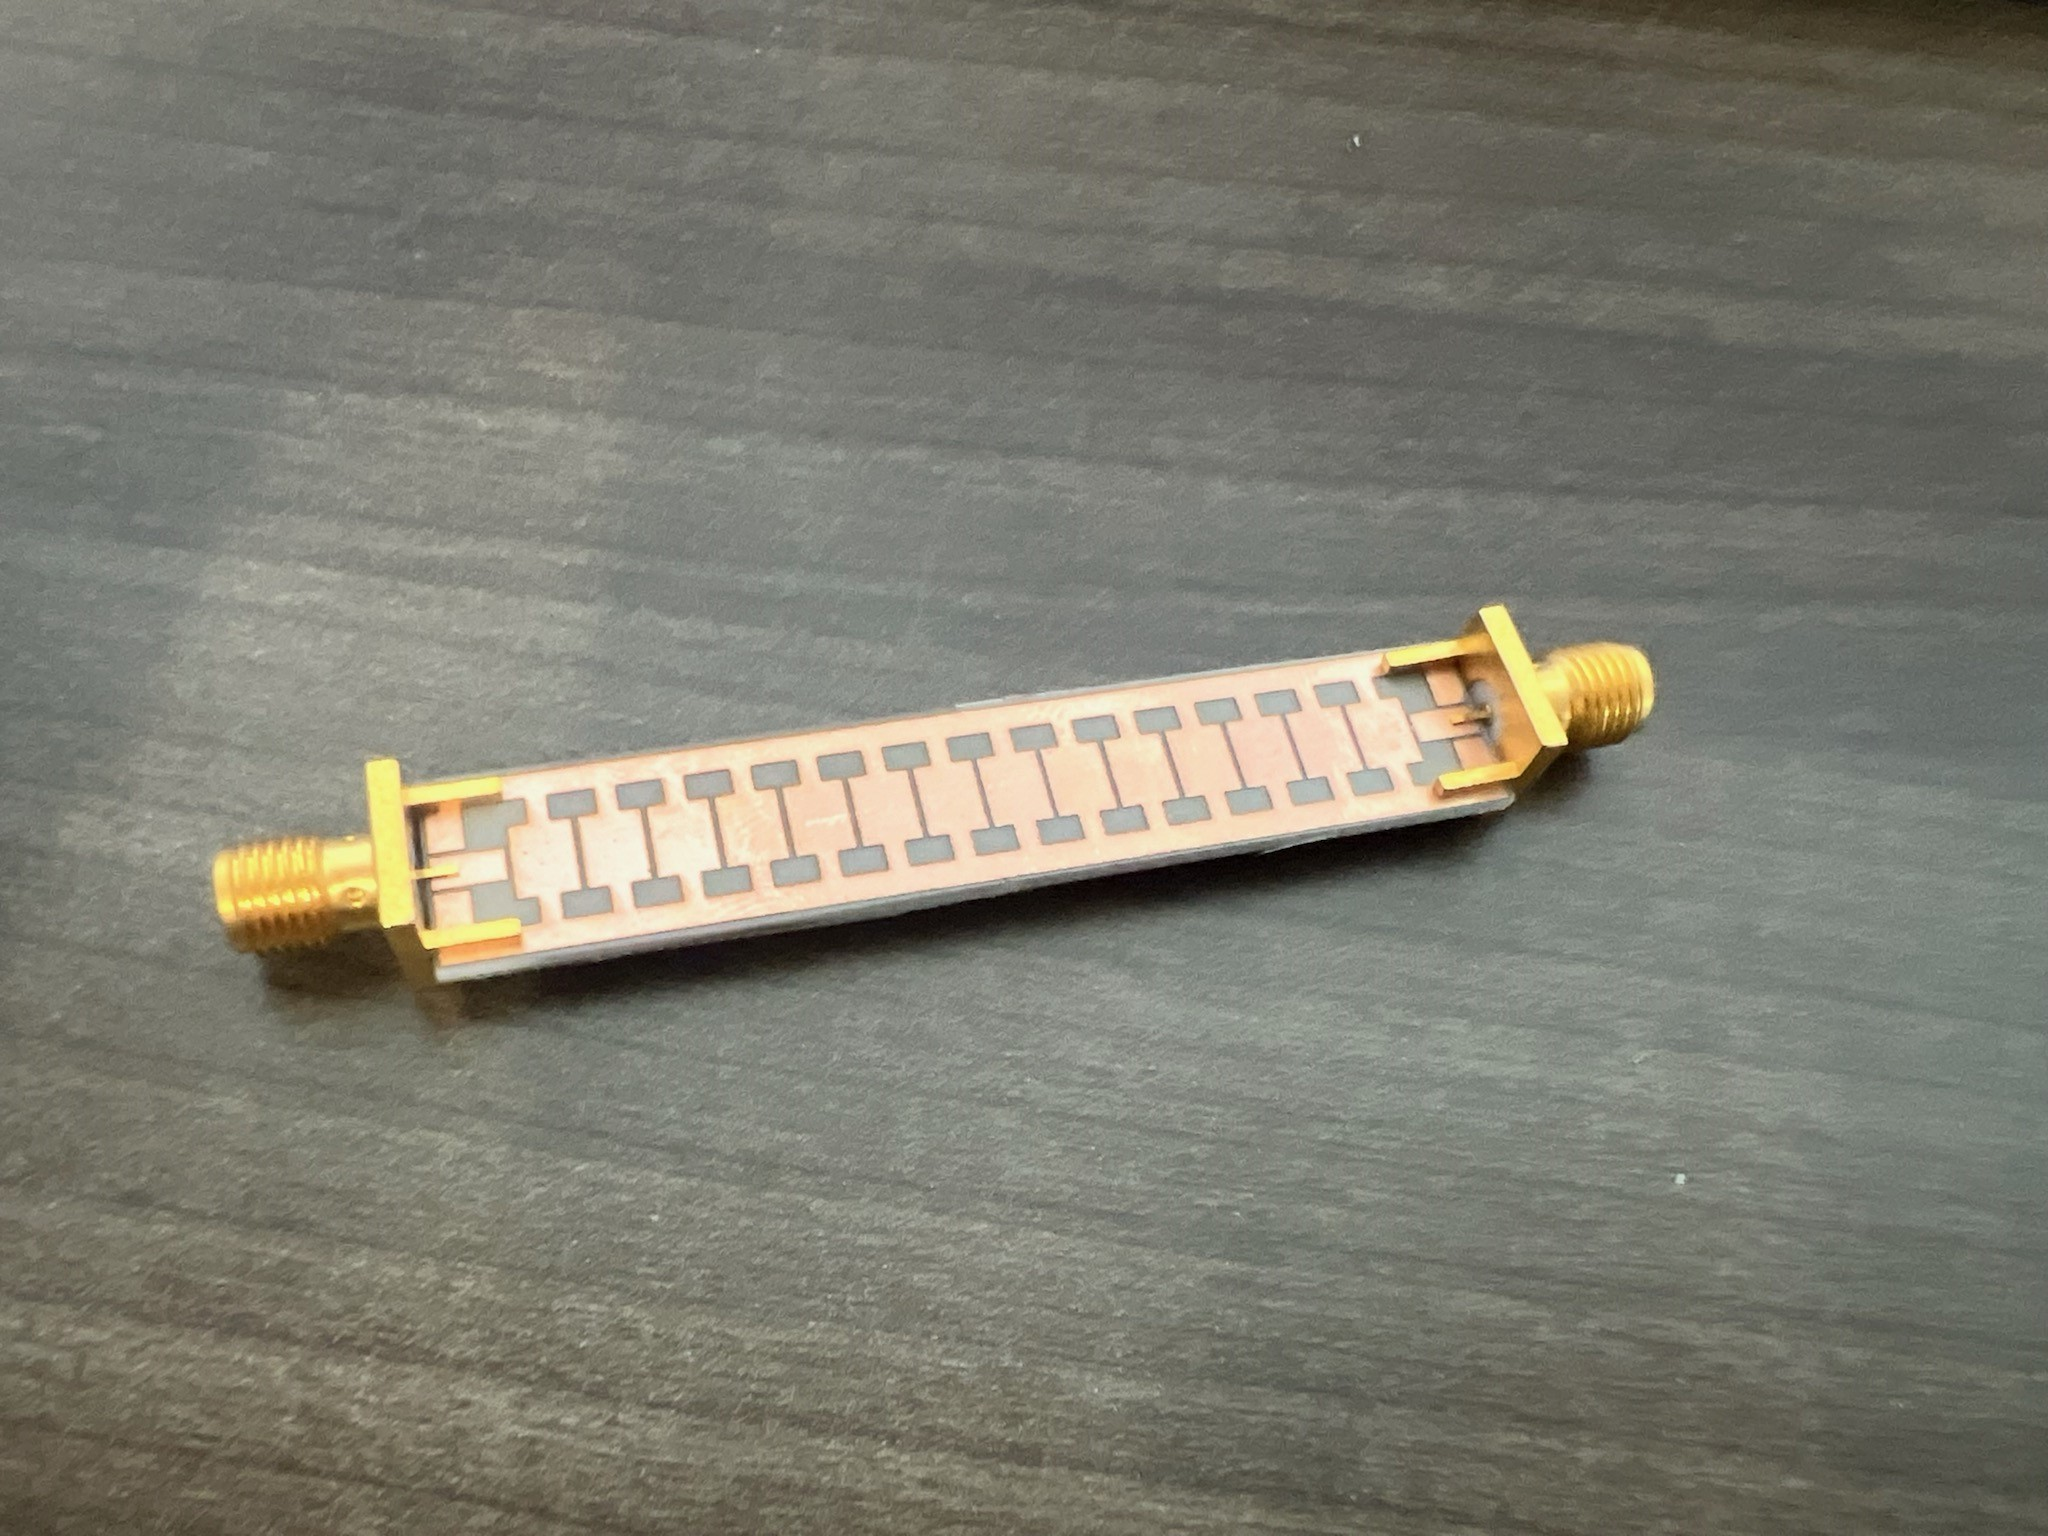
\includegraphics[width=2in]{manufactured_antenna}
    \captionof{figure}{Picture of Manufactured LWA}
    \label{manufactured_antenna_pic}
\end{Figure} 

After some analysis using the GUI, two geometries from the LWA were chosen to manufacture that met slightly different constraints, which are summarized in Table~\ref{manufactured_geometries_list}. The first antenna was selected before training the ML model on the additional data after performing the XAI analysis, and the second antenna was selected after. If the predictions were accurate, these antennas would perform very well within the desired constraints. Figure~\ref{manufactured_antenna_pic} shows what the first manufactured antenna looks like, and Figure~\ref{manufactured_antenna_performance} shows how the performance compared between the simulated and predicted $S_{11}$ values for each antenna. It was also planned to plot the measured performances from the manufactured antennas alongside the simulated and predicted values, but unforeseen issues during the antenna manufacturing process and time constraints prevented this. For the first manufactured antenna, the predictions seem to very closely follow the simulated values, with only slight variations. The second antenna has a less accurate prediction that fails to predict important antenna characteristics, such as the dip to -40 dB near 19.5 GHz. However, the simulated values proves that the predictions work well, since the antenna meets the original criteria of performing below -11.5 dB between 12.5 and 17 GHz.

\begin{Figure}
    \centering
    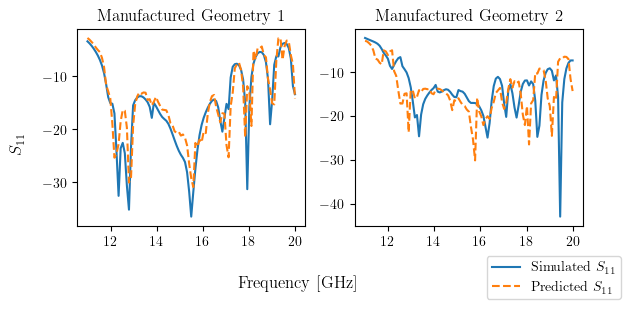
\includegraphics[width=3.5in]{manufactured_antenna_performance}
    \captionof{figure}{Manufactured LWA Performance}
    \label{manufactured_antenna_performance}
\end{Figure} 


\section{Conclusion}
Applying a ML algorithm as an aid in the process of optimizing antenna geometric parameters with EM simulations greatly reduces the amount of time and computational power required. Training a model on a small set of data obtained from running simulation software allows the model to fit to the trend of data. Large amounts of additional data can then be generated within the bounds of the existing data, and performance predictions can be made for this generated data with a decent accuracy. The most optimal geometries can be returned for specified performance values and frequency ranges, making the traditional way of relying on intuition and trial-and-error in order to determine which antenna geometries would allow for the best performance unnecessary. Additionally, open-source XAI libraries can then be applied to the model to allow for further analysis of the contribution each geometric feature makes to the predictions. After careful analysis of the weight that each parameter has on the overall model predictions using SHAP values, the most impactful parameters can be singled out to generate more simulations, which will be added to the ML model's training data. This will drive the accuracy even higher with the most minimal amount of simulations. 


\bibliographystyle{IEEEtran}
\bibliography{refs}

\vfill

\end{document}